\pagebreak
\section{Attachment}

\subsection*{Parameters of the WSCLEAN implementations}


\subsection*{Serial coordinate descent algorithm}

\subsubsection*{Efficient calculation of the Lipschitz constants}
In each iteration, we need the Lipschitz constant of the current pixel. I.e. we need the inner product $\langle PSF_{location}, PSF_{location} \rangle$ for every pixel. We can pre-calculate the Lipschitz constant before we run the serial coordinate descent algorithm. The naive way to calculate the Lipschitz constant for every pixel results in quadratic runtime(each inner product costs us $O(n)$ operations, and we do it for all $n$ pixels). But this is not necessary. We can pre-calculate the Lipschitz constant for every pixel in linear time.

Figure \ref{cd:efficient:lipschitz:padded} shows the $PSF$ shifted to a pixel location. The Lipschitz constant is by squaring all values of Figure \ref{cd:efficient:lipschitz:padded} and summing up the values. Or in another way: We sum up all the squared values of the $PSF$ inside a specific rectangle. All that changes for a Lipschitz calculation between different pixels is the specific rectangle.

\begin{figure}[h]
	\centering
	\begin{subfigure}[b]{0.3\linewidth}
		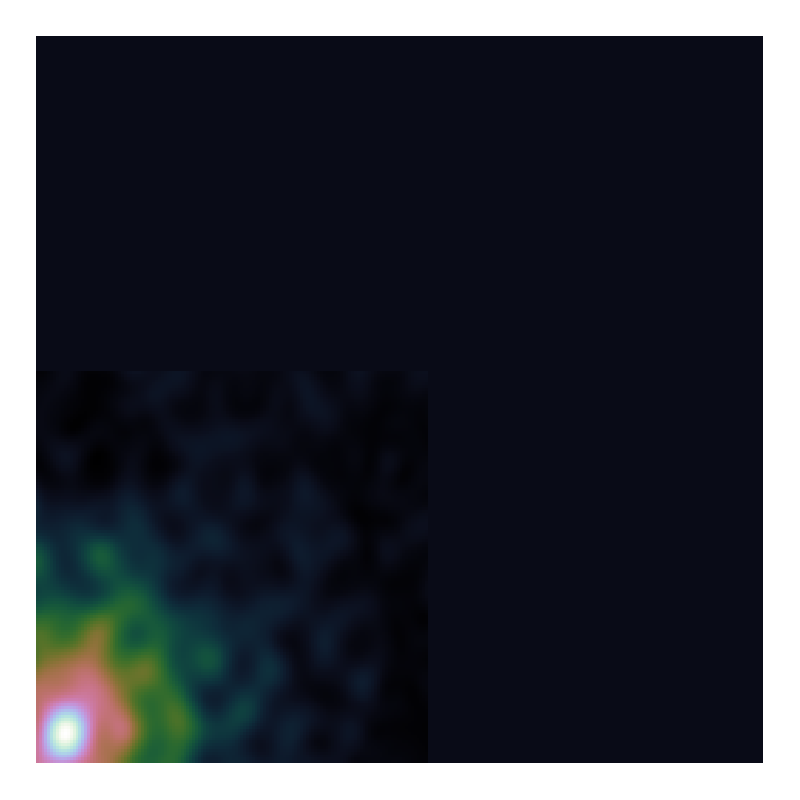
\includegraphics[width=\linewidth, clip, trim= 0.25in 0.25in 0.25in 0.25in]{./chapters/03.cd/simulated/psfZeroPadding.png}
		\caption{Shifted $PSF$.}
		\label{cd:efficient:lipschitz:padded}
	\end{subfigure}
	\begin{subfigure}[b]{0.3\linewidth}
		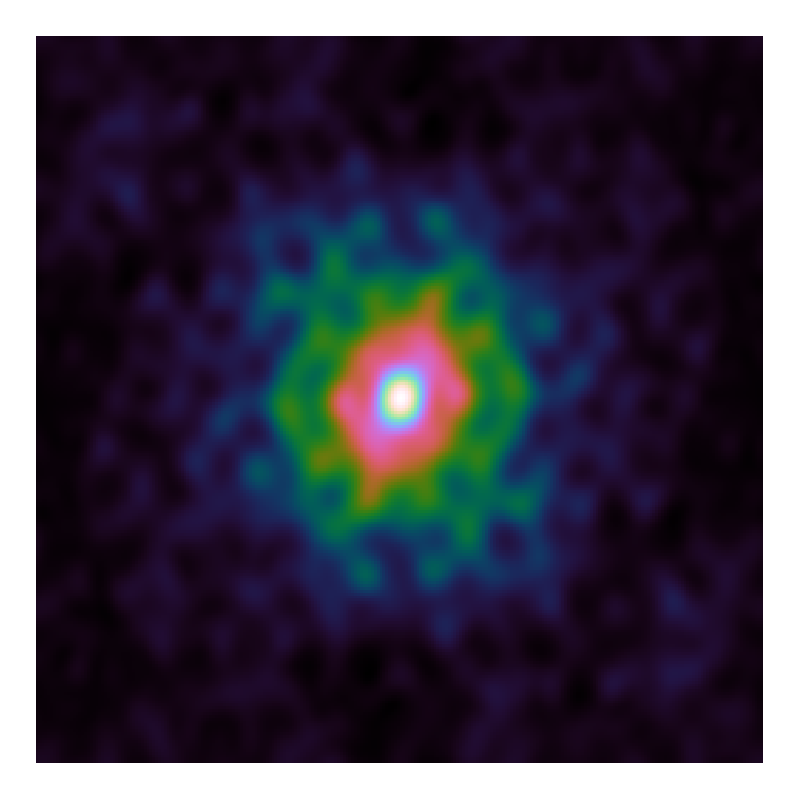
\includegraphics[width=\linewidth, clip, trim= 0.25in 0.25in 0.25in 0.25in]{./chapters/03.cd/simulated/psf.png}
		\caption{Sum of squared values.}
		\label{cd:efficient:lipschitz:rectangle}
	\end{subfigure}
	\caption{Sum of squared values for the Lipschitz constant.}
	\label{cd:efficient:lipschitz:figure}
\end{figure}

This can be exploited with a scan algorithm: We first calculate the result of every rectangle we can draw from the origin, up to some pixel value. We end up with an array we call $scan[,]$. It is the same size as the $PSF$, but contains the sum of squares inside a specific rectangle.

\begin{lstlisting}
var scan = new double[,];
for (i in (0, PSF.Length(0))
for (j in (0, PSF.Length(1))
var iBefore = scan[i - 1, j];
var jBefore = scan[i, j - 1];
var ijBefore = scan[i - 1, j - 1];
var current = PSF[i, j] * PSF[i, j];
scan[i, j] = current + iBefore + jBefore - ijBefore;
\end{lstlisting}

Every Lipschitz constant can be now calculated by combining the sums of different rectangles. Our example is shown in Figure \ref{cd:efficient:lipschitz:rectangle}. We start with the total sum of all values, and subtract two rectangles. Because the subtractions overlap, we need to add the third rectangle again. we take the total value. In short, we can calculate each Lipschitz constant by at most 4 lookups in the $scan[,]$ array.


\subsubsection*{GPU implementation}
We implemented the serial coordinate descent algorithm on the GPU. It is implemented in .Net Core with ILGPU\cite{ilgpu}. ILGPU is a Just-In-Time compiler for high performance GPU programs written in .Net Core.

GPU programs are split into kernels. Each kernel consists of a single routine optimized for executing on the GPU. Our serial coordinate descent algorithm consists of Step 1, find the best pixel to optimize, step 2, optimize pixel and then updating the gradient map. The GPU implementation of the Serial coordinate descent algorithm uses three kernels: Kernel 1 is equivalent to step 1. Kernel 2 updates the reconstruction $x$ and kernel 3 updates the gradient map.

Kernel 2 and 3 are straight forward to implement. The implementation of kernel 1, searching for the best pixel, is more interesting. Essentially, this step is a max reduce operation: We want to find the pixel with the maximum absolute step. We implemented the step 1 kernel with an atomic-max instruction:
\begin{lstlisting}
MaxPixelKernel(x, gradienstMap, lipschitz, location, maxPixel)
oldValue = x[location]
tmp = gradientsMap[location] + oldValue * lipschitzMap[location]
optimalValue = Max(tmp - lambda*alpha) / (lipschitz[location] + (1 - alpha)*lambda)
diff = optimalValue - oldValue
currentPixel = (absDiff = Abs(diff), diff = diff, location = location)
AtomicMax(maxPixel, currentPixel)
\end{lstlisting}

The kernel is executed on multiple processors in parallel on the GPU. Each processor is checking a single pixel. Communication is done with the atomic-max instruction. The atomic-max writes on a global variable, which keeps track of the current maximum pixel. This implementation turned out to be the fastest for the MaxPixelKernel. Warp shuffle\cite{keplerShuffle} was also tested, but resulted in a slower kernel.

Now to put the serial coordinate descent implementation on the GPU together, all we need to do is call the kernels, which perform the minimization on the GPU:


\begin{lstlisting}
do 
//Step 1: Search pixel
maxPixel = (absDiff = 0, diff = 0, location = (-1, -1))
ExecuteMaxPixelKernel(x, gradienstMap, lipschitz, maxPixel)
SynchronizeKernels()

//Step 2: Optimize
ExecuteUpdateXKernel(x, maxPixel.diff, maxPixel.location)
ExecuteUpdateGradientsKernel(gradientsMap, gradientUpdate, maxPixel.diff, maxPixel.location)
SynchronizeKernels()

while maxPixel.absDiff  < epsilon
\end{lstlisting}

Note that after each kernel call, we synchronize the program. We wait for all kernels on the GPU to be finished, before we continue with the next step. As we mentioned before, this is the core behind the serial coordinate descent algorithm. We have to wait for each step to finish before we can continue with the next. 


\subsubsection*{Distributed implementation MPI}
We created a distributed implementation of our serial coordinate descent algorithm using the Message Passing Interface (MPI). In MPI, we use several nodes of computers to solve the problem. Each node has its own processors an main memory, and we use MPI to communicate betweeen the nodes. 

We split the reconstructed image, and the gradient map into facets of equal size, and use one node for each facet. For example, our image is $1024^2$ pixels in size and we use 4 nodes. This means each node reconstructs a $512^2$ facet of the image, and has the matching $512^2$ entries of the gradient map locally. 

The distributed serial coordinate descent algorithm now searches the maximum pixel locally in each node. Then, all node agree on the best global pixel to optimize, which is an MPI\_ALLREDUCE operation. After MPI\_ALLREDUCE, each node knows the global pixel which gets minimized in this iteration. Then, each node updates its part of the gradient map locally.

This leads to the following pseudo-code algorithm:
\begin{lstlisting}
...
do 
oldObjectiveValue = objectiveValue

//Step 1: Search pixel
maxAbsDiff = 0
maxDiff = 0
pixelLocation = (-1, -1)
for(i in Range(0, dirty.Length(0))
for(j in Range(0, dirty.Length(1))
oldValue = x[i, j]
tmp = gradientsMap[i, j] + oldValue * lipschitzMap[i, j]
optimalValue = Max(tmp - lambda*alpha) / (lipschitz[i, j] + (1 - alpha)*lambda)
diff = optimalValue - oldValue

if(maxAbsDiff < Abs(diff))
maxAbsDiff = Abs(diff)
maxDiff = diff
pixelLocation = (i, j)

//communicate location with nodes
globalMaxAbsDiff, globalMaxDiff, globalLocation = MPI_ALLREDUCE(maxAbsDiff, maxDiff, pixelLocation)

//Step 2: Optimize pixel.
if(globalLocation == pixelLocation)
x[globalLocation] += globalMaxDiff

//housekeeping
shiftedUpdate = Shift(gradientUpdate, globalLocation)
gradientMap = gradientMap - shiftedUpdate * globalMaxDiff
while epsilon < maxAbsDiff
\end{lstlisting}

Each node in the distributed serial coordinate descent algorithm communicates its local pixel in each iteration. Meaning the distributed algorithm has a communication step in each serial coordinate descent iteration. The distributed algorithm only has to communicate a single pixel, but has to communicate often. This is a potential down-side of the implementation. Usually, distributed systems can speed up algorithms which communicate a large chunk of data rarely.

\subsubsection*{Serial coordinate descent speedup with MPI or GPU}\label{results:speedup}
In this section we test how much we can speed-up our serial coordinate descent algorithm by using distributed computing with MPI, or GPU acceleration.

We test the distributed serial coordinate descent on a shared memory system(Meaning all CPUs have access to the same main memory) with 32 CPUs. This is a best-case scenario for our implementation, because each node runs on the same physical machine: Our implementation needs a communication step between the nodes for each serial coordinate descent iteration. It needs a low-latency connection between each node to run as efficient as possible. Since each node runs on the same physical machine, it has a low latency times and therefore a low communication time. In this implementation, each node uses a single processor. We compare the speedup the algorithm achieves by adding more nodes/processors.

For the GPU we used personal computer level hardware, and tested on a nVidia Quadro M1200. We compare the speedup we achieve to the on-board CPU, which is an Intel Xeon E3-1505M with 8 logical processors at different image sizes. The speedup is shown in Figure \ref{results:speedup:figure}.

\begin{figure}[h]
	\centering
	\begin{subfigure}[b]{0.45\linewidth}
		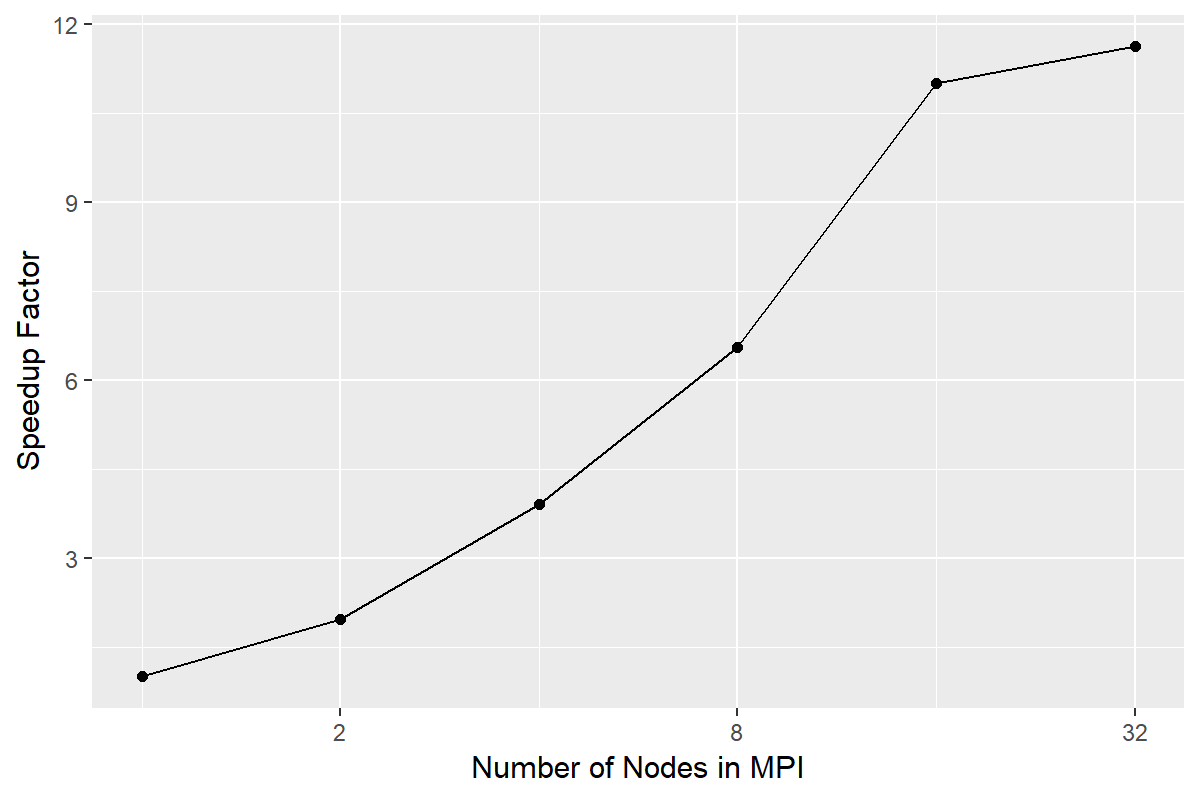
\includegraphics[width=1.00\linewidth]{./chapters/10.results/speedup/dist-speedup.png}
	\end{subfigure}
	\begin{subfigure}[b]{0.45\linewidth}
		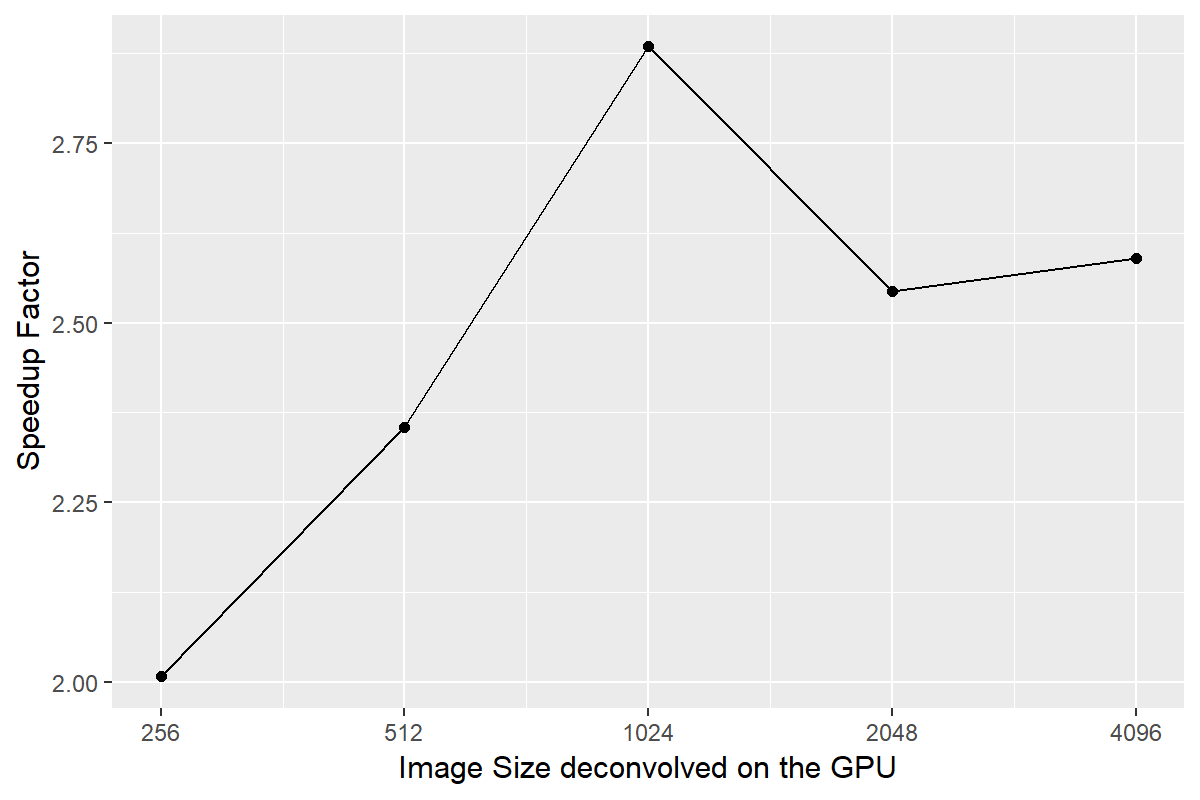
\includegraphics[width=1.00\linewidth]{./chapters/10.results/speedup/gpu.png}
	\end{subfigure}
	\caption{Speedup by using MPI or GPU acceleration}
	\label{results:speedup:figure}
\end{figure}

As we mentioned before, the speedup we achieve by using nodes/processors in MPI is the best-case scenario. As the best case scenario, we achieve a significant performance increase by using more nodes/processors. Up to 16 processors, the speedup we achieve is at least linear. Afterwards however the speedup diminishes. With 32 processors, we are only marginally faster than with 16. If the nodes would run two different physical machines, the speedup we achieve would depend mainly on the latency of the connection. 

The speedup we achieve by using GPU acceleration is fairly constant over the image size. The speedup factor varies around 2.5. Ideally, we would like to combine the distributed and the GPU implementation. However, this is not useful with the current implementation: The main bottleneck in the MPI implementation is the communication step in each iteration. 

We do not have a CLEAN implementation in our .Net Core pipeline. However, we mentioned the similarities between the serial coordinate descent and CLEAN in Section \ref{cd:similarities}. A single serial coordinate descent iteration is roughly equivalent to a standard CLEAN iteration. If we assume we need 14'000 CLEAN iterations to reconstruct an image, we can get a rough estimate by comparing the wall-clock time of 14'000 serial coordinate descent iterations. In this case, CLEAN is roughly 7 times faster than the current serial coordinate descent iteration.

Overall the serial coordinate descent algorithm with GPU acceleration is still several factors slower than CLEAN. The speedup we achieve with MPI is significant. But because serial coordinate descent and CLEAN have such a similar structure, we can expect a similar speedup with a CLEAN-MPI implementation. We need another method to speed up our deconvolution algorithm.


\subsection*{Parallel coordinate descent algorithm}

\subsubsection*{Block coordinate descent}
Instead of optimizing a single pixel in each iteration, the serial block coordinate descent algorithm can update a block of pixels. We start with the update rule of the serial coordinate descent algorithm, and show how it can be adapted to update a block of pixels in each iteration. Remember the single pixel update from the serial coordinate descent algorithm: 
\begin{equation} \label{pcdm:pcdm:block:single:update}
pixel_{opt} = \frac{max(gradient_{location} - \lambda\alpha, 0)}{Lipschitz_{location} + (1 - \alpha)\lambda}
\end{equation}

We optimize the pixel at the current location by taking the gradient and dividing it by the Lipschitz constant. For the block coordinate descent algorithm we vectorize the update rule: This means $gradient_{location}$ and $Lipschitz_{location}$ and the output $pixel_{opt}$ become vectors:

\begin{equation} \label{pcdm:pcdm:block:block:update}
pixels_{opt} = \frac{max(gradients_{locations} - \lambda\alpha, 0)}{Sum(Lipschitz_{locations}) + (1 - \alpha)\lambda}
\end{equation}

This is the serial block coordinate descent update rule. Note that we divide the gradient for each pixel by the the block Lipschitz constant (which is the sum of every pixel Lipschitz constant in the block). Note that the larger block we chose, the smaller the update becomes for each individual pixel inside the block. We have a central trade-off: We can take a large step for a single pixel, or take several smaller steps for a block of pixels. 

Remember: The Lipschitz constants for neighboring pixels have a similar value. Meaning for a block of $2^2 = 4$ pixels: $Sum(Lipschitz_{locations} \approx 4 Lipschitz$. Or less formally, we can either take a full step towards the minimum for a single pixel. Or if we update a block of $2^2$ pixels, we take $4$ $\frac{1}{4}$ steps towards the minimum.

The reader might be familiar with the (F)ISTA method\cite{beck2009fista}. The block update shown in equation \eqref{pcdm:pcdm:block:block:update} is related to the (F)ISTA update rule. When the block size equal to the image size (we update all pixels in the image in each iteration), then the serial block coordinate descent is equivalent to (F)ISTA.

The block update rule \eqref{pcdm:pcdm:block:block:update} allows us to minimize a single block of pixels in each iteration. But it comes with a trade-off: The bigger blocks we choose, the smaller steps we take for each individual pixel in the block. The reason why the serial block coordinate descent may be faster than the single pixel algorithm is when most pixels are correlated with their neighbors: Extended emissions have a large areas where the pixel values are correlated. Meaning if a pixel in the area is non-zero, then the neighboring pixels are also likely to be non-zero. A serial block coordinate descent algorithm can take more useful minimization steps in each iteration. We test different block sizes with our parallel algorithm in Section \ref{pcdm:results}. In our tests, different block sizes did not lead to a significant speedup.

\subsubsection*{Accelerated parallel block coordinate descent} \label{pcdm:pcdm:approx}
So far, we introduced the serial block coordinate descent and the ESO. The serial block coordinate descent can update a block of pixels in a single iteration, and the ESO estimates how much $PSF$s overlap when we perform parallel update steps. In this section, we put this together in an accelerated, parallel block coordinate descent algorithm based on APPROX\cite{fercoq2015accelerated}. But first, we introduce gradient acceleration.

In gradient acceleration, we use the gradient from previous iterations to speed up convergence of the current iteration. We can accelerate our serial coordinate descent algorithm by extending it with an acceleration parameter $\theta$, a copy of the gradient map and a copy of the reconstructed image $x$.  We term one couple of gradient map plus reconstructed image as 'explore', while the other couple is called 'correction'. The 'correction' gradient map and reconstructed image contain gradient information of the previous iterations. They are used to speed up the convergence of the 'explore'. In each iteration, the acceleration parameter $\theta$ decreases, and we use more information from the 'correction' gradient map and reconstruction.

This leads to the following accelerated, parallel and block coordinate descent deconvolution algorithm:
\begin{lstlisting}
dirty = IFFT(GridVisibilities(visibilities))
residualsPadded = ZeroPadding(dirty)

psfPadded = ZeroPadding(PSF)
psfPadded = FlipUD(FlipLR(psfPadded))
gradientUpdate = iFFT(FFT(ZeroPadding(PSF)) * FFT(psfPadded))

xExplore = new Array[,]
xCorrection = new Array[,]
gradientsMapExplore = iFFT(FFT(residualsPadded) * FFT(psfPadded))
gradientMapCorrection = new Array[,]
lipschitzMap = CalcLipschitz(PSF)

eso = ESO(CountNonZero(PSF), t, x.Length / blockSize)
theta0 = t / (x.Length / blockSize)
theta = theta0

do 
oldObjectiveValue = objectiveValue

//Step 1: select t blocks uniformly at random
blocks = sample(t)

//Step 2: update reconstruction in parallel
diffBlocks = new Array
parallel for each block in blocks
//increase blockLipschitz according to the ESO
blockLipschitz = Sum(GetBlock(LipschitzMap, block))
blockLipschitz = blockLipschitz * eso

oldBlock = GetBlock(xExplore, block)
tmp = theta^2 * GetBlock(gradientsMapCorrection, block) 
+ GetBlock(gradientsMapExplore, block) 
+ GetBLock(xExplore, block) * blockLipschitz
optimalBlock = Max(tmp - lambda*alpha) / (blockLipschitz + (1 - alpha)*lambda)
diffBlock = optimalBlock - oldBlock

xExplore[block] += diffBlock
xCorrection[block] += diffBlock * (-(1.0f - theta / theta0) / theta^2)
diffBlocks[block] = diffBlock

//Step 3: Update gradients
for each block in blocks
diffBlock = diffBlocks[block]
for each pixel in block
diff = diffBlock[pixel]
shiftedUpdate = Shift(gradientUpdate, pixelLocation)

gradientsMapExplore = gradientsMapExplore - shiftedUpdate * diff
gradientsMapCorrection = gradientsMapCorrection - shiftedUpdate * diff * (-(1.0f - theta / theta0) / theta^2)

theta = (Sqrt((theta^2 * theta^2) + 4 * (theta^2)) - theta^2) / 2.0f
while maxAbsDiff  < epsilon

output = new float[,]
for(i in in Range(0, dirty.Length(0))
for(j in in Range(0, dirty.Length(0))
output[i, j] = theta * xCorrection[i, j] + xExplore[i, j];
\end{lstlisting}

In each iteration, the parallel algorithm first samples $\tau$ unique blocks uniformly at random (we cannot select the same block more than in a single iteration). In the second step, we then update each block in parallel. Note that we multiply the block Lipschitz constant with the ESO, which ensures convergence for parallel updates. In the third step, we update the two gradient maps. The final image is a combination of the two reconstructed images $x$ from the 'explore' and 'correction' couple.

This algorithm is parallel, but it is still synchronized: It updates each block in parallel, but waits for all updates to finish before continuing with the next iteration. In the next Section \ref{pcdm:async}, we introduce an asynchronous implementation, where the individual processors do not wait for each other.

The accelerated, parallel coordinate descent algorithm reduces itself to a non-accelerated variant, if we do not modify $\theta$ in each iteration. In that case, the 'correction' gradient map and reconstruction $x$ stay zero over the course of the algorithm. Note that due to gradient acceleration, we need twice the memory (for the 'correction' maps), and twice the number of operations to update a single block. Gradient acceleration allows us to take larger steps towards the optimum in each iteration. As such, it should need fewer iterations to converge than the non-accelerated variant. But a single iteration of the accelerated variant is more expensive.

\subsubsection*{Active set heuristic}
The active set heuristic is typically used in cyclic coordinate descent: It chooses a subset of blocks, and optimizes the set until it converges. Then it chooses a  new set. We use the active set heuristic together with our pseudo-random selection strategy. A large portion of the blocks in the image will be zero. If we select blocks at pseudo-random, we are likely to select a block that will never contain non-zero values and we wasted computing resources by trying to update this block. The active set heuristic increases the likelihood that the pseudo-random strategy selects a relevant block. 

At the start of the parallel deconvolution algorithm, we initialize the active set by iterating over all blocks. We add all blocks which contain non-zero pixels, or pixels which may become non-zero by a serial coordinate descent iteration. Now during asynchronous parallel coordinate descent iterations, each processors only selects blocks from the active set. This increases the chance that each processor selects a block where pixel values can actually be modified.

Note that the algorithm only adds blocks to the active set, which can be changed to a non-zero value at the start of deconvolution. Over several iterations, there may be blocks that are not in the active set, but are part of the optimal solution. This is remedied with a restarting heuristic.


\subsubsection*{Restarting heuristic}
In accelerated gradient methods like APPROX or (F)ISTA, restarting the acceleration can lead to a significant speedup\cite{fercoq2016restarting}. In our accelerated variant, we use the current reconstructed image as the starting point, and reset the 'correction' gradient map and image $x$ to zero. The question is, at what point is it useful to restart our parallel coordinate descent algorithm?

We implemented two restarting strategies: One strategy is based on Glasmachers et al.\cite{glasmachers2014coordinate} and restarts the algorithm when the acceleration likely benefits from it. The other heuristic was developed by us and restarts the when the active set is likely to be missing blocks. There may be non-zero blocks in the image, which were not included when we initialized the active set. Our strategy estimates when the active set is likely missing relevant blocks, and restarts the algorithm with a new active set. In our tests, we always needed to restart due to the active set, and never due to the heuristic by Glasmachers. This is why we focus on our own developed restarting strategy, and ignore Glasmachers' in the pseudo-code.

Our own restarting heuristic is based on the following idea: We compare the maximum pixel difference after a number of asynchronous, parallel updates, to the difference a single step of serial block coordinate descent would produce. When the active set contains all relevant blocks, the parallel deconvolutions converge at a similar rate as the serial block coordinate descent. If the active set is missing important blocks, then the updates of the parallel coordinate descent start to converge, while the serial block coordinate descent update stays similar.

We extend the asynchronous parallel coordinate descent implementation with the active set and restarting heuristic:
\begin{lstlisting}
...
do
lastMaxDiff = GetGreedyMaxBlockDiff(gradientsMapExplore, xExplore)

parallelDiffFactor = 0
for activeSetIteration in activeSetIterations
parallelDiffs = new Array[]
...
//asynchronous iterations
...

maxParallelDiff = Max(parallelDiffs)

//restarting heuristic
if(parallelDiffFactor = 0)
parallelDiffFactor = lastMaxDiff / maxParallelDiff

currentMaxDiff = GetGreedyMaxBlockDiff(gradientsMapExplore, xExplore)
activeSetInvalid = lastAbsMax / maxParallelDiff > parallelDiffFactor * 2
activeSetInvalid = activeSetInvalid | currentMaxDiff > lastAbsMax & lastAbsMax / parallelDiffFactor > concurrentFactor
if activeSetInvalid
Restart()
parallelDiffFactor = 0
lastMaxDiff = currentMaxDiff
...
while lastMaxDiff  < epsilon
\end{lstlisting}

In each 'active set iteration', we let the asynchronous processors deconvolve the image for a set number of iterations. For example: Each processor deconvolves 1000 blocks asynchronously. If we use $\tau = 8 processors$, then this results in a single active set iteration consisting of 8000 asynchronous iterations. Remember that we are now using a pseudo-random strategy. After enough parallel iterations, we are practically guaranteed to have selected the same block as a single serial block coordinate descent algorithm, if it is contained in the active set.

After the first active set iteration, we save the factor of how much the parallel update how close the maximum parallel update is to the best greedy step. The ratio of maximum greedy update and maximum parallel update should stay similar over the course of the algorithm, if the active set is valid. If the active set invalid, if it is missing important blocks, the algorithm will encounter ever smaller values for $maxParallelDiff$, while $lastMaxDiff$ does not decrease significantly over the active set iterations. In that case, we restart the algorithm with a new active set.

In several tests, we also observed that the maximum greedy update may actually increase from one active set iteration to the next. This is possible when we were unlucky and did not select the maximum block within one of the many asynchronous iterations, or when the active set is invalid (the maximum block is not contained in the active set). In the latter case we want to restart the algorithm. This is why we added a more aggressive condition which flags the active set as invalid, if $currentMaxDiff$ increases over active set iterations.


\subsubsection*{Re-introduction of a 'Minor' cycles}
As we will demonstrate in Section \ref{results}, the parallel coordinate descent deconvolution algorithm benefits significantly from our $PSF$ approximation method. The drawback of our $PSF$ approximation is that it needs more major cycles to converge. We re-introduce a similar minor cycle to the Clark CLEAN algorithm \cite{clark1980efficient}, and reduce the number of necessary major cycles.

The CLEAN algorithm developed by Clark also uses only a fraction of the $PSF$ during CLEAN deconvolutions. After a number of iterations, the residuals of the Clark algorithm are inaccurate, and it resets the residuals with the full $PSF$. We use a similar idea: We run our parallel coordinate descent deconvolution algorithm and retrieve the intermediate solution. We then decide whether we reset the residuals using the full $PSF$ (the 'minor' cycle), or we use the major cycle.

Resetting the residuals with the full $PSF$ is done as follows:
\begin{lstlisting}
residuals = iFFT(Gridding(visibilities))  	//Major cycle
x = DeconvolveParallel(residuals, Cut(PSF)) 		//Deconvolve with approximate PSF
residuals_minor = residuals - iFFT(FFT(x) * FFT(PSF)) //Update with full PSF
\end{lstlisting}

We convolve the intermediate solution $x$ with the full $PSF$ in Fourier space, and subtract the result from the original residuals from the major cycle. This allows us to remove some of the errors which the $PSF$ approximation introduces, and reduce the number of Major cycles.

The question that remains is when to use a Major cycle or a 'Minor' cycle to reset the residuals. Remember from Section \ref{gradients}, we introduced a heuristic based on the $PSF$ side lobe: When we deconvolve using only a fraction of the full $PSF$, we leave side lobes in the residual image. In each major cycle, we can only run the deconvolution algorithm up to a certain point, before we include $PSF$ side lobes in the reconstructed image. In Section \ref{gradients} we created a path regularization, which estimates a $\lambda_{cycle}$ for each Major cycle. We used the largest $PSF$ side lobe (largest value not included in the $PSF$ window around the center) to estimate the minimum regularization $\lambda_{cycle}$ for each Major cycle.

Now with the addition of a 'Minor' cycle, we use the same path regularization twice: We have two minimum regularization parameters, $\lambda^{minor}_{cycle}$ and $\lambda^{major}_{cycle}$. The parameter $\lambda^{minor}_{cycle}$ decreases for each 'Minor' cycle, $\lambda^{major}_{cycle}$ decreases for each Major cycle. We  the 'Minor' cycle as long as $\lambda^{minor}_{cycle}$ is larger than $\lambda^{major}_{cycle}$. Otherwise, we start a new major cycle. We use the largest $PSF$ side lobe to estimate $\lambda^{minor}_{cycle}$ (the same as for the $\lambda_{cycle}$ before). For the second regularization parameter $\lambda^{major}_{cycle}$, we do not have a natural $PSF$ side lobe left in our approximation method. We chose to use the $PSF$ side lobe, which is outside the $\frac{1}{2}$ center window of the $PSF$ to estimate $\lambda^{major}_{cycle}$. 

In total, the major and 'Minor' cycle for our parallel coordinate descent algorithm is implemented as follows:
\begin{lstlisting}
residualVis = visibilities
x = new Array[,]

for each cycle in Range(0, maxMajorCycles)
residuals = iFFT(Gridding(residualVis))
residualsMinor = residuas

lambdaMajor = Estimate(residuals, PSF, 2)
lambdaMajor = Max(lambdaMajor, lambda)
lambdaMinor = 0

do
lambdaMinor = Estimate(residualsMinor, PSF, psfFraction)
lambdaMinor = Max(lambdaMinor, lambdaMajor)

x_current = DeconvolveParallel(residuals, Cut(PSF, psfFraction), lambdaMinor)
x + = x_current
residuals_minor = residuals - iFFT(FFT(x) * FFT(PSF))
while(lambdaMajor < lambdaMinor)

modelVis = DeGridding(FFT(x))
residualVis = visibilities - modelVis
\end{lstlisting}

In each 'Minor' cycle, we estimate the current $\lambda^{minor}_{cycle}$ regularization. We start the parallel coordinate descent algorithm with an approximate $PSF$ and the current $\lambda^{minor}_{cycle}$ regularization parameter. When the parallel algorithm has finished, we use the full $PSF$ to update the residuals. We restart the 'Minor' cycle if  $\lambda^{major}_{cycle} < \lambda^{minor}_{cycle}$.

An aggressive $PSF$ approximation leads to a sharp increase in the number of necessary Major cycles. With the re-introduction of 'Minor' cycles, we keep the total number of Major cycles comparable to other deconvolution algorithms like serial coordinate descent or CLEAN.

\subsubsection*{Block size}
The parallel coordinate descent algorithm can group several pixels in blocks, and optimize the blocks of pixels in parallel. It is not clear if grouping the pixels in blocks results in shorter convergence times. We test different block sizes in Figure \ref{pcdm:results:block}, all using the same $PSF$ approximation of $\frac{1}{32}$. We tested out block size of $1^2$ (every block contains a single pixel) up to a block size of $8^2$:

\begin{figure}[h]
	\centering
	\begin{subfigure}{0.6\linewidth}
		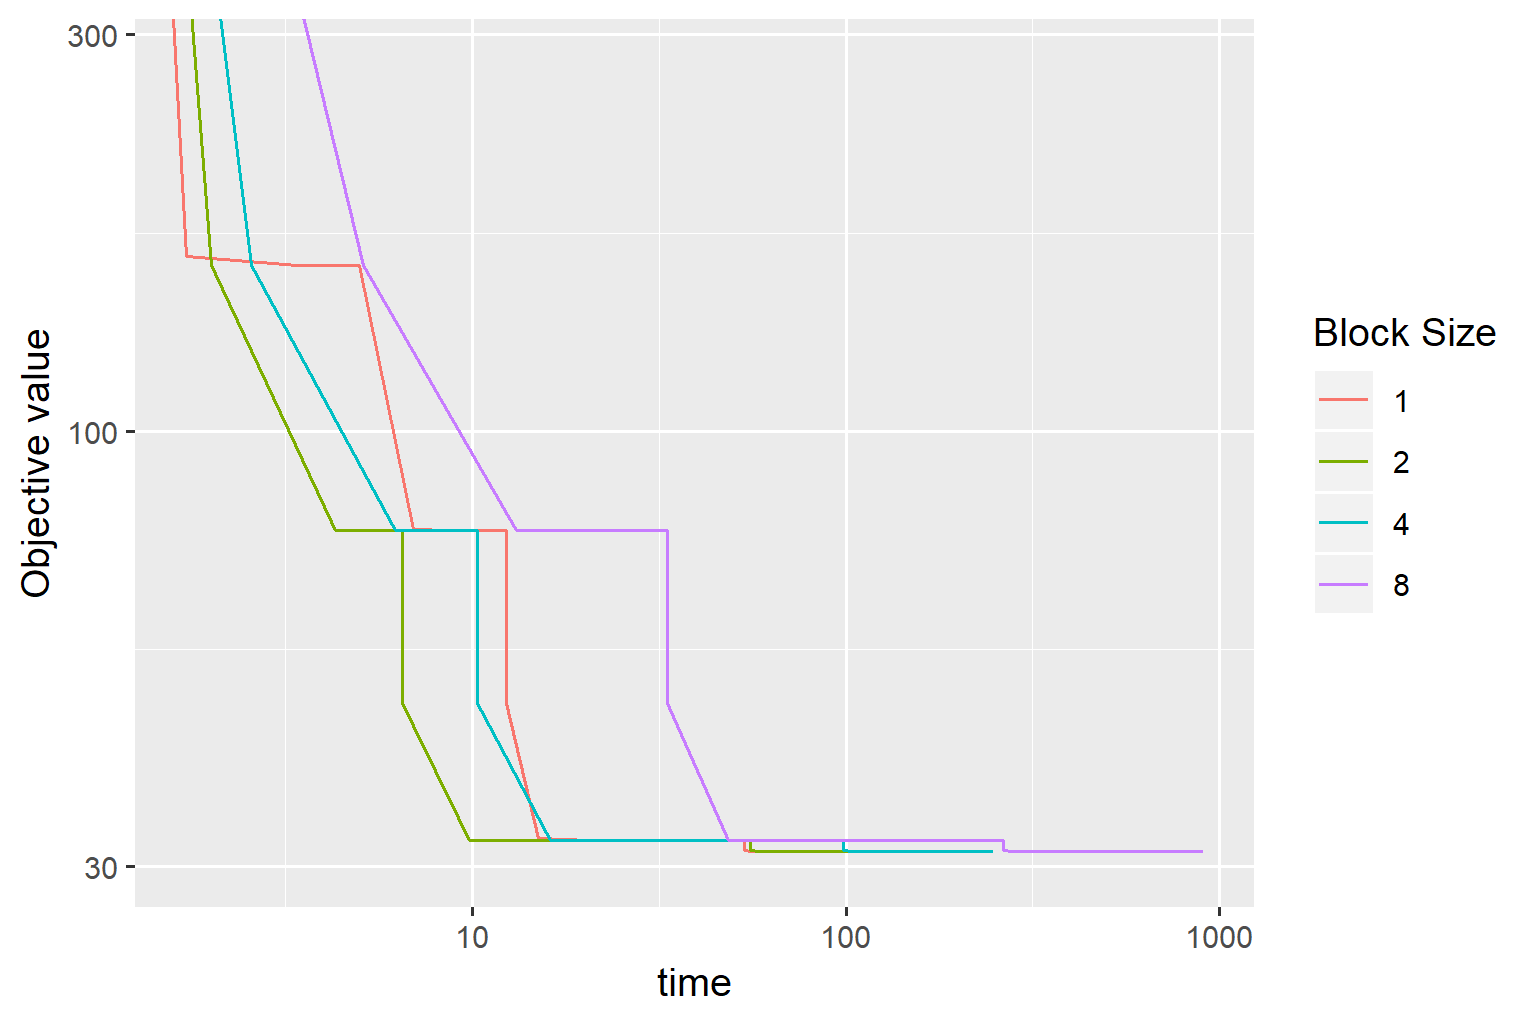
\includegraphics[width=1.0\linewidth]{./chapters/05.pcdm/parameters/blockSize.png}
	\end{subfigure}
	\begin{subfigure}{0.35\linewidth}
		\begin{tabular}{c | r}
			Block Size & Total seconds \\ \hline
			$1^2$ & 108 \\
			$2^2$ & 103 \\
			$4^2$ & 248 \\
			$8^2$ & 905 \\
		\end{tabular}
	\end{subfigure}
	\caption{Convergence times with different block sizes}
	\label{pcdm:results:block}
\end{figure}

The larger block sizes of $4^2$ and $8^2$ are significantly slower to converge than a block size of $1^2$. Only a block size of $2^2$ is slightly faster. Interestingly though, the parallel coordinate descent algorithm is faster to arrive at intermediate results with the block sizes $2^2$ and $4^2$. This suggests that the parallel coordinate descent algorithm may benefit starting out from larger block sizes, and gradually reducing the block size over several major cycle iterations.

However, two factors lead to the decision to simply use a block size of $1^2$ for all major cycle iterations: First, the block size is likely connected to the image resolution. An effective heuristic that starts with larger blocks may become difficult to develop for general observations. Secondly, the parallel coordinate descent implementation becomes more complicated when it has to account for different block sizes. An implementation with a block size of only $1^2$ is shorter and simpler.

For the rest of this project, we use a block size of $1$, meaning every thread is minimizing a single pixel.


\subsubsection*{Acceleration}
Lastly, we test whether the parallel coordinate descent algorithm is faster with or without gradient acceleration. The accelerated variant needs two versions of the gradient map, which get updated asynchronously with compare-exchange operations. Figure \ref{pcdm:results:acc} compares the accelerated and non-accelerated parallel coordinate descent algorithm.

\begin{figure}[h]
	\centering
	\begin{subfigure}{0.6\linewidth}
		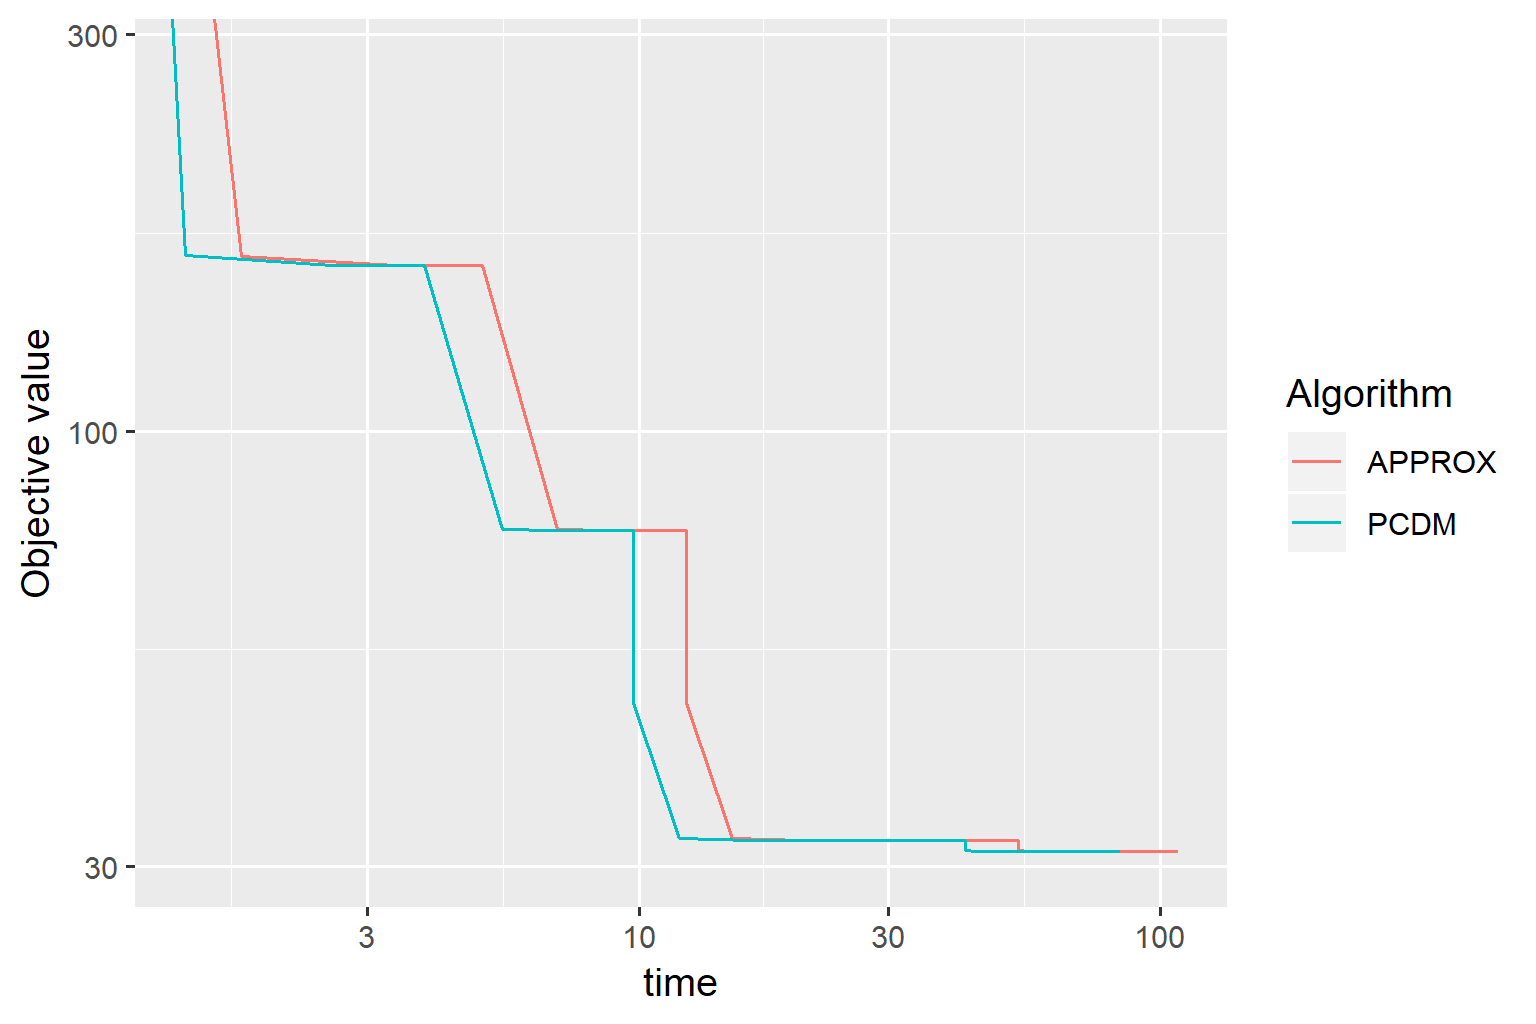
\includegraphics[width=1.0\linewidth]{./chapters/05.pcdm/parameters/acceleration.png}
	\end{subfigure}
	\begin{subfigure}{0.35\linewidth}
		\begin{tabular}{c | c}
			Method & Total seconds \\ \hline
			With Acceleration & 108 \\
			Without Acceleration & 84 \\
		\end{tabular}
	\end{subfigure}
	\caption{Convergence time with or without gradient acceleration.}
	\label{pcdm:results:acc}
\end{figure}

The accelerated variant is significantly slower in every part of the algorithm. Our hypothesis is that the two gradient maps necessary for the acceleration also increase the cost of synchronization.

Furthermore the accelerated variant has additional run time costs which were not measured in this test: It has to create a copy of the gradient map and the reconstructed image for the acceleration. Meaning this test shown in Figure \ref{pcdm:results:acc} is biased in favor of the accelerated variant, yet it is still slower.

\pagebreak
